 
\section{Pri kio temas}

%%%>>>>>>>>>>>>>>>>>>>>>>>>>>>>>>>>>>>>>>>>>>>>>>>>>>>>>>>>>>>>>>>>>>>>>>>>>>>>>>>>>>>>>>>>>>>>>>
  \begin{frame}
    \frametitle{La interkona lumbildo}
    
  	\setbeamercovered{transparent}
    Levu la manojn kiu:

	\begin{itemize}
		
		\item<1-1> Agas en iu ajn organizo

		\item<2-2> Agas en iu ajn esperanta organizo
		
		\item<3-3> Agas en landa sekcio
				
	\end{itemize}
	
  \end{frame}
%%%<<<<<<<<<<<<<<<<<<<<<<<<<<<<<<<<<<<<<<<<<<<<<<<<<<<<<<<<<<<<<<<<<<<<<<<<<<<<<<<<<<<<<<<<<<<<<<



%%%>>>>>>>>>>>>>>>>>>>>>>>>>>>>>>>>>>>>>>>>>>>>>>>>>>>>>>>>>>>>>>>>>>>>>>>>>>>>>>>>>>>>>>>>>>>>>>
  \begin{frame}
    \frametitle{Pri la trejnado}

  	\setbeamercovered{transparent}
	
	\begin{itemize}

		\item<-1> Ĝi celas proponi al via organizo ilon kaj metodon kiel plezure kunlabori.
		
		\item<-1> Mi tamen ne ofendiĝos se al vi ne plaĉos la ideo, estu verdirema.
		
		\item<2-2> Mi koncentriĝos sur praktikaj aspektoj de aplikado al~E-organizo~--~pri~teĥnikaĵoj oni povas legi multon en Interreto.
	
		\item<2-2> Neniu montrota ekzemplo estas artefarita. Ĉiuj devenas de lastjara funkciado de Pola Esperanto-Junularo.
		
		\item<3-3> Tiuspeca esperanta trejnado okazas la unuan fojon. Memoru fuŝojn, difektojn kaj helpu plibonigi. Antaŭdankon!
				
		\item<3-3> Prezentaĵo kunmetita en \LaTeX
				
	\end{itemize}
  \end{frame}
%%%<<<<<<<<<<<<<<<<<<<<<<<<<<<<<<<<<<<<<<<<<<<<<<<<<<<<<<<<<<<<<<<<<<<<<<<<<<<<<<<<<<<<<<<<<<<<<<


\subsection{Problemo?}

%%%>>>>>>>>>>>>>>>>>>>>>>>>>>>>>>>>>>>>>>>>>>>>>>>>>>>>>>>>>>>>>>>>>>>>>>>>>>>>>>>>>>>>>>>>>>>>>>
  \begin{frame}
    \frametitle{Komenco}
    \framesubtitle{Vi havas 20 novajn mesaĝojn.}
    
  \begin{center}
    	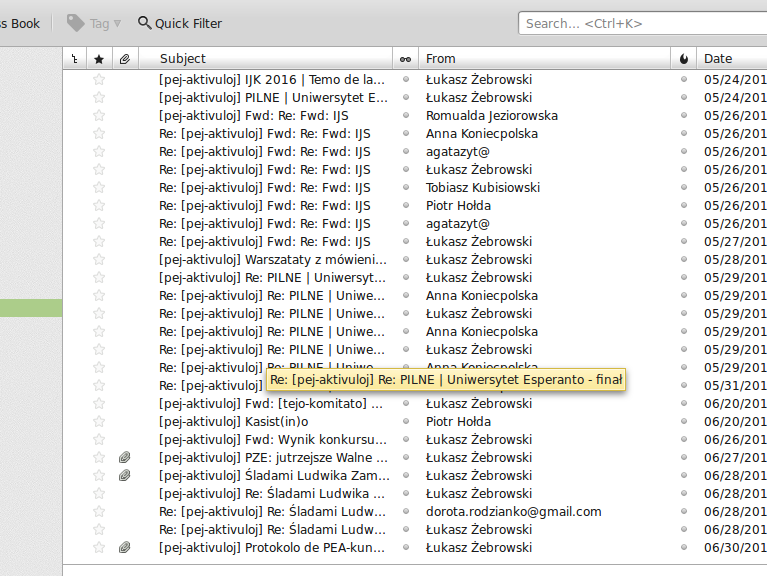
\includegraphics[scale=0.3]{ekranoj/retposhto}
	\end{center}
  \end{frame}
%%%<<<<<<<<<<<<<<<<<<<<<<<<<<<<<<<<<<<<<<<<<<<<<<<<<<<<<<<<<<<<<<<<<<<<<<<<<<<<<<<<<<<<<<<<<<<<<<
 

%%%>>>>>>>>>>>>>>>>>>>>>>>>>>>>>>>>>>>>>>>>>>>>>>>>>>>>>>>>>>>>>>>>>>>>>>>>>>>>>>>>>>>>>>>>>>>>>>
  \begin{frame}
    \frametitle{Retpoŝto}
    \framesubtitle{Ĉu vi ŝatas ĝin uzi por esperantaj projektoj?}
    \begin{itemize}
    	\item Kiom da retadresoj vi uzas?
    	\item Kiom da esperanto-rilataj (nepersonaj = malinteresaj) mesaĝoj vi ricevas semajne?
    	\item Kiom da el ili rilatas rekte al vi?
    	\item Ĉu vi ĉiam (iam ajn?) tuj recivinte la mesaĝon plenumas peton/taskon aŭ prokrastetas?
    \end{itemize}
  \end{frame}
%%%<<<<<<<<<<<<<<<<<<<<<<<<<<<<<<<<<<<<<<<<<<<<<<<<<<<<<<<<<<<<<<<<<<<<<<<<<<<<<<<<<<<<<<<<<<<<<<
   
   
\subsection{Solvopropono}
   
%%%>>>>>>>>>>>>>>>>>>>>>>>>>>>>>>>>>>>>>>>>>>>>>>>>>>>>>>>>>>>>>>>>>>>>>>>>>>>>>>>>>>>>>>>>>>>>>>    
  \begin{frame}
    \frametitle{Taskolistoj?}

   	\begin{center}
	   	
\includegraphics[scale=0.5]{meme/to_do_list}
   	\end{center}
    
    \begin{itemize}
    	\item Ĉu vi ilin uzas por organizi sian ĉiutagan laboron?
    	\item Kiel tio helpas?
    \end{itemize}
        
  \end{frame}    
%%%<<<<<<<<<<<<<<<<<<<<<<<<<<<<<<<<<<<<<<<<<<<<<<<<<<<<<<<<<<<<<<<<<<<<<<<<<<<<<<<<<<<<<<<<<<<<<<


   
%%%>>>>>>>>>>>>>>>>>>>>>>>>>>>>>>>>>>>>>>>>>>>>>>>>>>>>>>>>>>>>>>>>>>>>>>>>>>>>>>>>>>>>>>>>>>>>>>
  \begin{frame}
    \frametitle{Taskolistoj!}
    %http://www.learningcommons.uoguelph.ca/guides/time_management/html/making_task_list.html
    Aldone:
    \begin{itemize}
    	\item Helpas memori eĉ pri flankaj taskoj.
     	\item Oni povas taksi la prioritatojn = sukcesi ĝis limdatoj
        \item Malpli da prokrastado, ĉar vi havos realecan imagon kiom da laboro vere farendas.      
    \end{itemize}
  \end{frame}      
%%%<<<<<<<<<<<<<<<<<<<<<<<<<<<<<<<<<<<<<<<<<<<<<<<<<<<<<<<<<<<<<<<<<<<<<<<<<<<<<<<<<<<<<<<<<<<<<<

   
%%%>>>>>>>>>>>>>>>>>>>>>>>>>>>>>>>>>>>>>>>>>>>>>>>>>>>>>>>>>>>>>>>>>>>>>>>>>>>>>>>>>>>>>>>>>>>>>>
  \begin{frame}
    \frametitle{La propono: Trello.com}
    \begin{center}
    	
\includegraphics[scale=0.4]{bildoj/trello}
    \end{center}    
  \end{frame}
%%%<<<<<<<<<<<<<<<<<<<<<<<<<<<<<<<<<<<<<<<<<<<<<<<<<<<<<<<<<<<<<<<<<<<<<<<<<<<<<<<<<<<<<<<<<<<<<<
  
%%%>>>>>>>>>>>>>>>>>>>>>>>>>>>>>>>>>>>>>>>>>>>>>>>>>>>>>>>>>>>>>>>>>>>>>>>>>>>>>>>>>>>>>>>>>>>>>>
  \begin{frame}
    \frametitle{Kial -- la bildoj sinesprimas.}
    \framesubtitle{Elektu!}
    
	\begin{columns}
    \column{0.5\textwidth}
	    \begin{center}
    		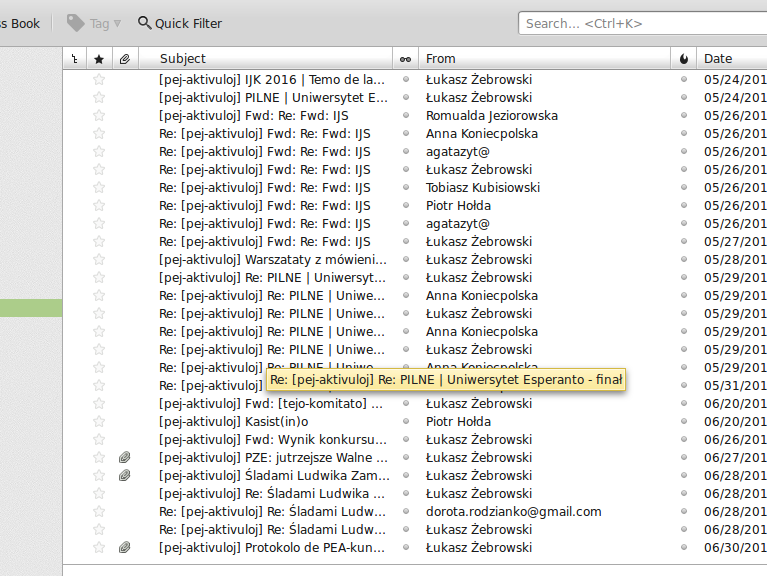
\includegraphics[scale=0.2]{ekranoj/retposhto}
    	\end{center}
	\column{0.5\textwidth}
    	\begin{center}
    	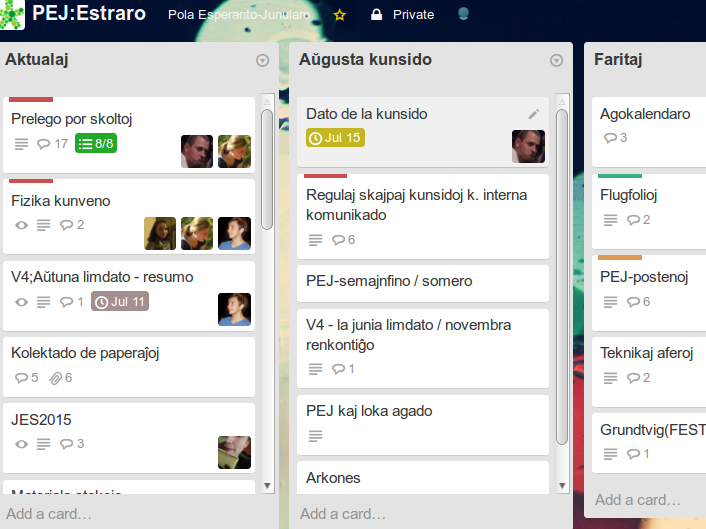
\includegraphics[scale=0.22]{ekranoj/trello-bonas-estraro}
    	\end{center}

	\end{columns}
  \end{frame}
%%%<<<<<<<<<<<<<<<<<<<<<<<<<<<<<<<<<<<<<<<<<<<<<<<<<<<<<<<<<<<<<<<<<<<<<<<<<<<<<<<<<<<<<<<<<<<<<<



%%%>>>>>>>>>>>>>>>>>>>>>>>>>>>>>>>>>>>>>>>>>>>>>>>>>>>>>>>>>>>>>>>>>>>>>>>>>>>>>>>>>>>>>>>>>>>>>>
  \begin{frame}
    \frametitle{Trello - kiu ĝin uzas?}
    
    \begin{itemize}
    	\item programistoj (kompreneble),
    	\item komercistoj por kunlabori,
    	\item sciencistoj por masturmi siajn esplorojn,
    	\item instruistoj por komuniki kun lernantoj,
    	\item iu verkisto por organizi verkadon de sia libro,
    	\item Junulara E-Semajno organizantoj.
    \end{itemize}
    
  \end{frame}
%%%<<<<<<<<<<<<<<<<<<<<<<<<<<<<<<<<<<<<<<<<<<<<<<<<<<<<<<<<<<<<<<<<<<<<<<<<<<<<<<<<<<<<<<<<<<<<<<
  

%%%>>>>>>>>>>>>>>>>>>>>>>>>>>>>>>>>>>>>>>>>>>>>>>>>>>>>>>>>>>>>>>>>>>>>>>>>>>>>>>>>>>>>>>>>>>>>>>
  \begin{frame}
    \frametitle{Ne nur Trello}
    \frametitle{Ekzistas multaj similaj sistemoj!}
    
    	\begin{itemize}
    		\item \textbf{Asana}: pagenda, pli riĉa (do samtempe komplika), ne tiom vidklara
    		\item \textbf{basecamp}: miaopinie maltaŭga por e-organizoj
    	\end{itemize}
  \end{frame}
%%%<<<<<<<<<<<<<<<<<<<<<<<<<<<<<<<<<<<<<<<<<<<<<<<<<<<<<<<<<<<<<<<<<<<<<<<<<<<<<<<<<<<<<<<<<<<<<<

